\documentclass{article}

\usepackage{graphicx} %[pdftex] OR [dvips]
\usepackage{fullpage}
\usepackage{float}
\usepackage{titling}
\setlength{\droptitle}{-6em}

\newcommand{\ghcfile}[1]{\textsl{#1}}

\title{Implementing Backpack}

\begin{document}

\maketitle

The purpose of this document is to describe an implementation path
for Backpack~\cite{Kilpatrick:2014:BRH:2535838.2535884} in GHC\@.

We start off by outlining the current architecture of GHC, ghc-pkg and Cabal,
which constitute the existing packaging system.  We then state what our subgoals
are, since there are many similar sounding but different problems to solve.  Next,
we describe the ``probably correct'' implementation plan, and finish off with
some open design questions.  This is intended to be an evolving design document,
so please contribute!

\section{Current packaging architecture}

The overall architecture is described in Figure~\ref{fig:arch}.

\begin{figure}[H]
    \center{\scalebox{0.8}{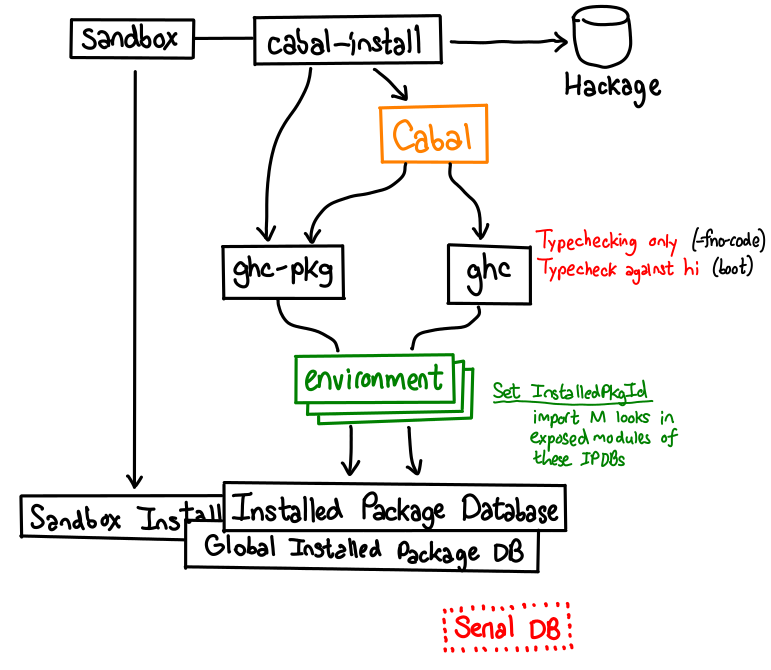
\includegraphics{arch.png}}}
\label{fig:arch}\caption{Architecture of GHC, ghc-pkg and Cabal. Green bits indicate additions from upcoming IHG work, red bits indicate additions from Backpack.  Orange indicates a Haskell library.}
\end{figure}

Here, arrows indicate dependencies from one component to another.  Color
coding is as follows: orange components are libaries, green components
are to be added with the IHG work, red components are to be added with
Backpack.  (Thus, black and orange can be considered the current)

\subsection{Installed package database}

Starting from the bottom, we have the \emph{installed package database}
(actually a collection of such databases), which stores information
about what packages have been installed are thus available to be
compiled against.  There is both a global database (for the system
administrator) and a local database (for end users), which can be
updated independently.  One way to think about the package database
is as a \emph{cache of object code}.  In principle, one could compile
any piece of code by repeatedly recompiling all of its dependencies;
the installed package database describes when this can be bypassed.

\begin{figure}[H]
    \center{\scalebox{0.8}{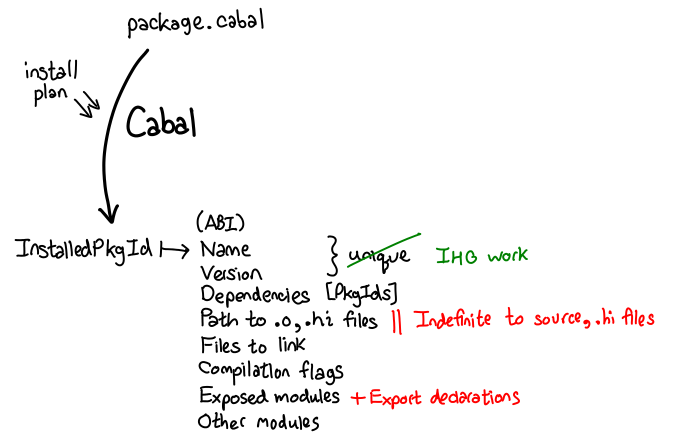
\includegraphics{pkgdb.png}}}
\label{fig:pkgdb}\caption{Anatomy of a package database.}
\end{figure}

In Figure~\ref{fig:pkgdb}, we show the structure of a package database.
The installed package are created from a Cabal file through the process
of dependency resolution and compilation.  In database terms, the primary key
of a package database is the InstalledPackageId
(Figure~\ref{fig:current-pkgid}).  This ID uniquely identifies an
instance of an installed package.  The PackageId omits the ABI hash and
is used to qualify linker exported symbols: the current value of this
parameter is communicated to GHC using the \verb|-package-id| flag.

In principle, packages with different PackageIds should be linkable
together in the same compiled program, whereas packages with the same
PackageId are not (even if they have different InstalledPackageIds).  In
practice, GHC is currently only able to select one version of a package,
as it clears out all old versions of the package in
\ghcfile{compiler/main/Package.lhs}:applyPackageFlag.

\begin{figure}
    \center{\begin{tabular}{r l}
        PackageId & package name, package version \\
        InstalledPackageId & PackageId, ABI hash \\
    \end{tabular}}
\label{fig:current-pkgid}\caption{Current structure of package identifiers.}
\end{figure}

The database entry itself contains the information from the installed package ID,
as well as information such as what dependencies it was linked against, where
its compiled code and interface files live, its compilation flags, what modules
it exposes, etc.  Much of this information is only relevant to Cabal; GHC
uses a subset of the information in the package database.

\subsection{GHC}

The two programs which access the package database directly are GHC
proper (for compilation) and ghc-pkg (which is a general purpose
command line tool for manipulating the database.)  GHC relies on
the package database in the following ways:

\begin{itemize}
    \item It imports the local and global package databases into
        its runtime database, and applies modifications to the exposed
        and trusted status of the entries via the flags \verb|-package|
        and others (\ghcfile{compiler/main/Packages.lhs}).  The internal
        package state can be seen at \verb|-v4| or higher.
    \item It uses this package database to find the location of module
        interfaces when it attempts to load the module info of an external
        module (\ghcfile{compiler/iface/LoadIface.hs}).
\end{itemize}

GHC itself performs a type checking phase, which generates an interface
file representing the module (so that later invocations of GHC can load the type
of a module), and then after compilation projects object files and linked archives
for programs to use.

\subsection{hs-boot}

\verb|hs-boot| is a special mechanism used to support recursive linking
of modules within a package, today.  Suppose I have a recursive module
dependency between modules and A and B. I break one of\ldots

(ToDo: describe how hs-boot mechanism works)

\subsection{Cabal}

Cabal is the build system for GHC, we can think of it as parsing a Cabal
file describing a package, and then making (possibly multiple)
invocations to GHC to perform the appropriate compilation.  What
information does Cabal pass onto GHC\@?  One can get an idea for this by
looking at a prototypical command line that Cabal invokes GHC with:

\begin{verbatim}
ghc --make
    -package-name myapp-0.1
    -hide-all-packages
    -package-id containers-0.9-ABCD
    Module1 Module2
\end{verbatim}

There are a few things going on here.  First, Cabal has to tell GHC
what the name of the package it's compiling (otherwise, GHC can't appropriately
generate symbols that other code referring to this package might generate).
There are also a number of commands which configure its in-memory view of
the package database (GHC's view of the package database may not directly
correspond to what is on disk).  There's also an optimization here: in principle,
GHC can compile each module one-by-one, but instead we use the \verb|--make| flag
because this allows GHC to reuse some data structures, resulting in a nontrivial
speedup.

(ToDo: describe cabal-install/sandbox)

\section{Goals}

There are actually a number of different goals we have for modifying the
packaging system, some of which are subsets of the Backpack system.

\begin{itemize}
    \item As a prerequisite, support multiple instances of containers-2.9 \emph{in the
        package database}.  These instances may be compiled against
        different dependencies, have the same dependencies but different
        source files (as when a package is being developed), or be
        compiled with different options.  It is less important to allow
        these instances to be linkable together.\footnote{Actually, I think
        this is completely orthogonal to Backpack, since we are going to treat
        dependencies as part of the package ID, so they would be considered
        separate entries in the package database anyway.}

    \item Support typechecking a library against a module interface
        as opposed to an actual implementation.  This would be useful
        for moving towards a model where Cabal package dependency versions
        are replaced with proper signature packages. %  See Section~\ref{sec:signature-packages} for more details.

    \item Support compiling the aforementioned libraries with actual implementations.
        It is \emph{not} a goal to be able to compile a library while only
        partially providing dependencies, and it is low priority to support
        mutually recursive implementations of these implementations.

        \iffalse%
    \item Support insertion of backwards compatibility shims for packages
        that are using old versions of packages, so that you can continue
        using them without having to patch them manually.  This is a
        stylized use-case of Backpack features.  See Section~LINKME for
        more details.

    \item Some easy-to-implement subset of the functionality provided by
        packages with holes (Backpack proper).  This includes support
        of linking an executable containing multiple packages with the
        same package name but different PackageIds.
        \fi
\end{itemize}

A lower priority goal is to actually allow multiple instances of
containers-2.9 to be linked together in the same executable
program.\footnote{In particular, this requires changes to how linker
symbols are assigned. However, this feature is important to
implement a number of Backpack features.}

A \emph{non-goal} is to allow users to upgrade upstream libraries
without recompiling downstream. This is an ABI concern and we're not
going to worry about it.

\section{Aside: Recent IHG work}\label{sec:ihg}

The IHG project has allocated some funds to relax the package instance
constraint in the package database, so that multiple instances can be
stored, but now the user of GHC must explicitly list package-IDs to be
linked against.  In the far future, it would be expected that tools like
Cabal automatically handle instance selection among a large number of
instances, but this is subtle and so this work is only to do some
foundational work, allowing a package database to optionally relax the
unique package-version requirement, and utilize environment files to
select which packages should be used.  See Duncan's email for more
details on the proposal.

To implement this:

\begin{enumerate}

    \item Remove the ``removal step'' when registering a package (with a flag)

    \item Check \ghcfile{compiler/main/Packages.lhs}:mkPackagesState to look out for shadowing
      within a database. We believe it already does the right thing, since
      we already need to handle shadowing between the local and global database.

\end{enumerate}

Once these changes are implemented, we can program multiple instances by
using \verb|-hide-all-packages -package-id ...|, even if there is no
high-level tool support.

Actually, this concern is orthogonal to the purposes of Backpack, if
we redefine PackageId appropriately.

\paragraph{The ABI hash} Currently, InstalledPackageId
is constructed of a package, version and ABI hash
(generateRegistrationInfo in
\ghcfile{libraries/Cabal/Cabal/Distribution/Simple/Register.hs}).  The
use of an ABI hash is a bit of GHC-specific hack introduced in 2009,
intended to make sure these installed package IDs are unique.  While
this is quite clever, using the ABI is actually a bit inflexible, as one
might reasonably want to have multiple copies of a package with the same
ABI but different source code changes.\footnote{In practice, our ABIs
are so unstable that it doesn't really matter.}

In Figure~\ref{fig:proposed-pkgid}, there is an alternate logical
representation of InstalledPackageId which attempts to extricate the
notion of ABI compatibility from what actually might uniquely identify a
package beyond its PackageId.  We imagine these components to be:

\begin{itemize}
    \item A hash of the source code (so one can register different
        in-development versions without having to bump the version
        number);
    \item Compilation way (profiling? dynamic?)
    \item Compilation flags (such as compilation way, optimization,
        profiling settings)\footnote{This is a little undefined on a package bases, because in principle the flags could be varied on a per-file basis. More likely this will be approximated against the relevant fields in the Cabal file as well as arguments passed to Cabal.};
\end{itemize}

A historical note: in the 2012 GSoC project to allow multiple instances
of a package to be installed at the same time, use of \emph{random
numbers} was used to workaround the inability to get an ABI early
enough.  We are not using this plan.

\section{Infrastructural improvements}

There are some infrastructural improvements that must be made before
Backpack proper can be implemented.  These additions are described in
red in the architectural diagrams.  The current structure of this
section is to describe the additions bottom up.

\subsection{Concrete physical identity = PackageId$^*$ + Module name}\label{sec:ipi}

\begin{figure}
    \center{\begin{tabular}{r l}
        PackageId & hash of ``package name, package version, PackageIds of dependent packages'' \\
        InstalledPackageId & hash of ``PackageId, source code, way, compiler flags'' \\
    \end{tabular}}
\label{fig:proposed-pkgid}\caption{Proposed new structure of package identifiers.}
\end{figure}

In Backpack, there needs to be some mechanism for assigning
\emph{physical module identities} to modules, which are essential for
typechecking Backpack packages, since they let us tell if two types are
equal or not. In the paper, the physical identity was represented as the
package that constructed it as well as some representation of the module
source.  We can simplify this slightly: in current Cabal packages, we
require that modules always be given a package-unique logical name;
thus, physical identities can be simply represented as a PackageId plus
module name. (See \ghcfile{compiler/basicTypes/Module.lhs:Module})
In fact, this coincides with how GHC already internally handles
the problem of type equality: it appeals to an \emph{original name}
which is, presently, a PackageId and the module name.

However, with the current representation of PackageIds, this is
insufficient: a package is not just its name, but also the regular
tree representing all of its package dependencies.  Thus, we have
to adjust the representation of a PackageId so that it includes this
regular tree, as seen Figure~\ref{fig:proposed-pkgid}.  Since this
tree in general may be quite long, it needs to be shortened in some way,
such as by hashing.

And now, the complications\ldots

\paragraph{Relaxing package selection restrictions}  As mentioned
previously, GHC is unable to select multiple packages with the same
package name (but different PackageIds).  This restriction needs to be
lifted.  For backwards compatibility reasons, it's probably better to
not overload \verb|-package-id| but add a new flag, maybe \verb|-force-package-id|;
we also need to disable the old version masking behavior.  This is orthogonal
to the IHG work, which wants to allow multiple InstalledPackageIds in the
\emph{database} (here, we want to allow multiple PackageIds in compiled code).

\paragraph{Linker symbols} As we increase the amount of information in
PackageId, it's important to be careful about the length of these IDs,
as they are used for exported linker symbols (e.g.
\verb|base_TextziReadziLex_zdwvalDig_info|).  Very long symbol names
hurt compile and link time, object file sizes, GHCi startup time,
dynamic linking, and make gdb hard to use.  As such, the current plan is
to do away with full package names and versions, and instead use just a
base-62 encoded hash, perhaps with the first four characters of the package
name for user-friendliness.

Edward: I'm still partial to a short hash of the dependency bits (or
even Simon's registry of short strings to dependency trees), and keeping
everything else the same.

\paragraph{Wired-in names} One annoying thing to remember is that GHC
has wired-in names, which refer to packages without any version.  Now
these wired names also have to accomodate dependency trees. A
suggested approach is to have a fixed table from these wired names to
package IDs; alternately we can use something like the special \verb|inplace|
version number.

\paragraph{Free variables (or, what is a non-concrete physical
identity?)} Physical identities in their full generality are permitted
to have free variables, which represent holes.  Handling this is a
tricky question, and we defer it to Section~\ref{sec:variables}, when
we talk about packages with holes.

\subsection{Exposed modules should allow external modules}\label{sec:reexport}

In Backpack, the definition of a package consists of a logical context,
which maps logical module names to physical module names.  These do not
necessarily coincide, since some physical modules may have been defined
in other packages and mixed into this package.  This mapping specifies
what modules other packages including this package can access.
However, in the current installed package database, we have exposed-modules which
specify what modules are accessible, but we assume that the current
package is responsible for providing these modules.

To implement Backpack, we have to extend this exposed-modules (``Export declarations''
on Figure~\ref{fig:pkgdb}).  Rather
than a list of logical module names, we provide a new list of tuples:
the exported logical module name and original physical module name (this
is in two parts: the InstalledPackageId and the original module name).
For example, an traditional module export is simply (Name, my-pkg-id, Name);
a renamed module is (NewName, my-pkg-id, OldName), and an external module
is (Name, external-pkg-id, Name).

\section{Simplifying Backpack}\label{sec:simplifying-backpack}

Backpack as currently defined always requires a \emph{shaping} pass,
which calculates the shapes of all modules defined in a package.
The shaping pass is critical to the solution of the double-vision problem
in recursive module linking, but it also presents a number of unpalatable
implementation problems:

\begin{itemize}

    \item A shaping pass means that it's not possible to compile modules
        in a package one-by-one, even if there is \emph{no mutual
        recursion} at all in the package.  Without mutual recursion, the
        shaping pass should not be necessary.  (Maybe this is not true!)
        Always enforcing two-passes means Backpack is not a ``pay as you
        go'' language feature.

    \item The calculated module shapes are quite intricate: in particular,
        they contain information about the providences of all data types
        and identifiers defined by a module.  To run a shape analysis, we
        must preprocess and parse all modules\ldots and then parse them
        again later, in the second, type-checking pass; furthermore, all
        of this information must be passed to GHC later.

    \item The conclusions of the shaping pass are \emph{incompatible} with
        what types of mutual recursion GHC can actually compile today
        via hs-boot: primarily, GHC requires that any data type or function
        defined in an hs-boot file also be \emph{defined} in its corresponding
        hs file. (In this way, we can assign an original name to it immediately,
        which simplifies compilation immensely.)

    \item The mode of program organization Backpack encourages, mutually
        recursive modules, is less efficient than code without recursive
        dependencies: thus programmers have good motivation to avoid
        this design pattern when possible.

\end{itemize}

The shaping pass is fundamentally necessary for some types of Backpack packages.
Here is the example which convinced Simon:

\begin{verbatim}
package p where
    A :: [data T; f :: T -> T]
    B = [export T(MkT), h; import A(f); data T = MkT; h x = f MkT]
    A = [export T(MkT), f, h; import B; f MkT = MkT]
\end{verbatim}

The key is to observe that B \emph{may or may not typecheck} depending
on the definition of A. Because A reexports B's definition T, B will
typecheck; but if A defined T on its own, B would not typecheck.  Thus,
we \emph{cannot} typecheck B until we have done some analysis of A (the
shaping analysis!)

All of these restrictions point to the desirability of a subset of
Backpack which does not allow mutually recursive modules, and
consequently does not require a shaping pass.

Here is the programming discipline, called the \textbf{linking restriction}: \emph{Module implementations
must be declared before signatures.}  Alternately, $+ \oplus - \neq - \oplus +$.  Here's an example:

\begin{verbatim}
package random where
    System.Random = [ ... ].hs

package monte-carlo where
    System.Random :: ...
    System.MonteCarlo = [ ... ].hs
\end{verbatim}

Now, to link these two applications together, only one ordering
is permissible:

\begin{verbatim}
package myapp where
    include random
    include monte-carlo
\end{verbatim}

or even (if myapp wants to provide its own random library):

\begin{verbatim}
package myapp2 where
    System.Random = [ ... ].hs
    include monte-carlo
\end{verbatim}

That is, all of \verb|monte-carlo|'s holes have been filled in by the time
it is included.  The alternate ordering is not allowed, as it could have
resulted in a recursive 

Why does this discipline prevent mutually recursive modules?  Intuitively,
the signature is the mechanism by which we can get a handle on an implementation
before it is defined, thus allowing circularity. If there is never an earlier handle
to an implementation, circularity is not possible.  A simple example of
this violation is in the reordered version of \verb|myapp2|:

\begin{verbatim}
package myapp2 where
    include monte-carlo
    System.Random = [ import System.MonteCarlo ].hs
\end{verbatim}

(Nota bene: this restriction applies to aliasing to, which can induce
linking as well).

\subsection{Why isn't shaping necessary?}

(ToDo: have this formally setup and everything)

In the case that we are compiling a definite package (there will be no leftover
holes), the argument is quite simple.  In vanilla Backpack, when a
signature is defined, we have to generate a pile of module variables
which may get unified with physical module identities.  However, with
the linking restriction, we only ever link a signature with a
\emph{fully instantiated} module definition. Thus, all module variables
can be immediately eliminated, and all we need to do is maintain an
updating logical context (i.e., module environment) so that later
modules know how to resolve imports.

When we are typechecking an indefinite package (there may be leftover
holes), things are a little more subtle.  When a signature is defined,
we \emph{know} that it will never be unified against a proper module
name.  So we can assign it some fresh original name.

Edward: What I find a bit dodgy is that there still are circumstances
where we will link a signature with a signature.  For example, if I have:

\begin{verbatim}
package a where
    A :: [ data A ]
    B :: [ data A ]
    M = ...
    A = B
    Q = ...
\end{verbatim}

We haven't violated the linking rule, but if we chose separate original
names for A and B, they need to be identified after the alias.

Fortunately, Q should typecheck as if the As are the same, but M should
typecheck as if they are distinct.  There is some ordering here, and our
claim (to be formally verified) is that these unifications can be
resolved as we process them.

\subsection{Installing indefinite packages}\label{sec:indefinite-packages}

If an indefinite package contains no code at all, we only need
to install the interface file for the signatures.  However, if
they include code, we must provide all of the
ingredients necessary to compile them when the holes are linked against
actual implementations.  (Figure~\ref{fig:pkgdb})

\paragraph{Source tarball or preprocessed source?}  An ancillary design choice
to be made is what the representation of the source that is saved is.  There
are a number of possible choices:

\begin{itemize}
    \item The original tarballs downloaded from Hackage,
    \item Preprocessed source files,
    \item Some sort of internal, type-checked representation of Haskell code (maybe the output of the desugarer).
\end{itemize}

Storing the tarballs is the simplest and most straightforward mechanism,
but we will have to be very certain that we can recompile the module
later in precisely the same we compiled it originally, to ensure the hi
files match up (fortunately, it should be simple to perform an optional
sanity check before proceeding.) The appeal of saving preprocessed
source, or even the IRs, is that this is conceptually this is exactly
what an indefinite package is: we have paused the compilation process
partway, intending to finish it later. It allows us to reuse the work
done preprocessing or typechecking.  However, it may be the case that
these phases work differently once library dependencies are known; typechecking
especially, see Section~\ref{sec:variables}.

\subsection{Compilation}

When we need to compile an indefinite package (since all of its
dependencies have been found), there seem to be two implementation
strategies possible.  Here is a very simple example to consider for the
various cases:

\begin{verbatim}
package pkg-a where
    A = ...
package pgk-b where -- indefinite package
    A :: ...
    B = [ b = ... ]
package pkg-c where
    include pkg-a
    include pkg-b
\end{verbatim}

\paragraph{The ``downstream'' proposal}  This is Simon's favorite
proposal.  Because of the linking invariant, if we traverse the Backpack
specification, any given module we need to compile will have all of its
dependencies compiled (since it could only depend on the dependency if
there was a signature, and the signature could not have been linked
unless it was implemented previously.)  So we just go ahead and compile
everything one-by-one, as if the package was a single big package.  (Of
course, if we encounter a definite package, don't bother recompiling
it; just use it directly.)  In
particular, we maintain the invariant that any code generated will
export symbols under the current package's namespace.  So the identifier
\verb|b| in the example becomes a symbol \verb|pkg-c_pkg-b_B_b| rather
than \verb|pkg-b_B_b| (package subqualification is necessary because
package C may define its own B module after thinning out the import.)

One big problem with this proposal is that it doesn't implement applicative
semantics.  If there is another package:

\begin{verbatim}
package pkg-d where
    include pkg-a
    include pkg-b
\end{verbatim}

this will generate its own instance of B, even though it should be the same
as C.  Simon was willing to entertain the idea that, well, as long as the
type-checker is able to figure out they are the same, then it might be OK
if we accidentally generate two copies of the code (provided they actually
are the same).

\paragraph{The ``upstream'' proposal}
The problem with the ``downstream'' proposal is that it always recompiles
all of the indefinite parts of the package, even if some of them should
be shared in some sense.  Hypothetically, a fully linked version of an
indefinite package should be considered a package in its own right
(in particular, it is associated with a physical module identity in Backpack).
So all we need to do is store these installed packages somewhere, probably
the local package database.  If we recompile the same dependency chain,
the installed package can be simply reused.  These products do not have
to be exposed.

One problem with this proposal is in this previous example:

\begin{verbatim}
package myapp2 where
    System.Random = [ ... ].hs
    include monte-carlo
\end{verbatim}

Here, monte-carlo depends on a ``subpart of the myapp2 package'', and it's
not entirely clear how to express this.

\subsection{Restricted recursive modules ala hs-boot}

It should be possible to support GHC-style mutual recursion using the
Backpack formalism immediately using hs-boot files.  However, to avoid
the need for a shaping pass, we must adopt an existing constraint that
already applies to hs-boot files: \emph{at the time we define a signature,
we must know what the original name for all data types is}.  We then
compile modules as usual, but compiling against the signature as if it
were an hs-boot file.

(ToDo: Figure out why this eliminates the shaping pass)

Compiling packages in this way gives the tantalizing possibility
of true separate compilation: the only thing we don't know is what the actual
package name of an indefinite package will be, and what the correct references
to have are.  This is a very minor change to the assembly, so one could conceive
of dynamically rewriting these references at the linking stage.

\iffalse%

\section{Module variables and original names}\label{sec:variables}

In Backpack, the physical identities of modules are in fact trees of
variables, constructors and recursive module identities.  As we
mentioned in Section~\ref{sec:ipi}, for concrete modules where there are
no free variables, physical identity maps nicely to an original name.
For packages with holes, the original names mechanism needs to be more
flexible; we need to first run a shaping pass in order to figure out if
a module is actually equal to another.

The direct approach is to replace original names with Backpack's
physical identities and use unification to do comparisons.  However,
this would require extremely invasive changes to all aspects of GHC, as
the original names assumption is baked quite deeply into the compiler:
we'd like to avoid upsetting this applecart if possible.

One key insight is that when we can only compile when all of the holes
are eliminated; thus all parts of the compilation pipeline beyond
typechecking can, in fact, assume that they will only be dealing with
concrete module identities.  One interpretation of this fact is that
we might actually be able to implement unification properly.

This gives us more latitude for how to
deal with the identities during typechecking: we may, for example,
adopt a conservative analysis (or an optional, dangerously liberal one),
secure in the knowledge that when we compile the final concrete module,
we will typecheck again with everything put together properly.

The next subsection describes one proposal for dealing with this issue,
and in what ways it is unsound.  We imagine there are other strategies

\subsection{Holes have physical module identities associated with definition site}

When compiling a module with a hole, we create a set of interface files
from the signature.  In the current architecture of GHC, we implicitly
assume that all interface files are associated with an \emph{original
name} (see below); thus, this means that it is very natural to assign an
original name to every hole.  If we have a signature package:

\begin{verbatim}
package foo-1x-sig where
    Foo :: ...
\end{verbatim}

Then the physical identity associated with Foo would be
\verb|foo-1x-sig_Foo| (rather than a fresh module variable $\alpha$).

This has implications for signature linking. Take this example from
Section 2.3 of the Backpack paper:

\begin{verbatim}
package yourlib where
    Prelude :: [data List a = ...]
    Yours :: [import Prelude; ...]

package mylib where
    Prelude :: [data Bool = ...]
    include yourlib
    Mine = [import Prelude; import Yours; ...]
\end{verbatim}

The first order of business is that we have to merge the interfaces of
the two Prelude holes, which are associated with different generated
physical identities (\verb|yourlib_Prelude| and \verb|mylib_Prelude|),
and furthermore, \emph{assign an original name to it}.  If we pick,
for example, \verb|mylib_Prelude|, none of the types defined in \verb|yourlib|
will unify in \verb|Mine|; thus, we would need to rename the original names
in \verb|yourlib|.\footnote{Edward: I don't think this is really the
right way to talk about this: Backpack requires a shaping pass and we should
be talking about it}

% ezyang: So, I thought I knew what I was talking about here, but actually
% the text here needs to be put in the context of shaping, so I need to
% think about this some more

\paragraph{Instantiation and reuse}

If we only ever linked any written signature with a signle implementation, this would actually
be great: when it is time to properly compile a module with holes, we
type check against the true original name of the new module (and just
do a consistency check between the signature and the implementation, modulo
differences in the physical identity)---a case of typechecking proceeding
differently between the initial typecheck and final compilation.

However, conflating a variable with an original name is very bad business.
Consider the graph library 

However, Backpack supports the linking of two signatures together, which
now presents a formidable difficulty: the original names of these two
signatures now must be identified.  Here is a real-world example where
this shows up:

\begin{verbatim}
package foo-1x-sig where
    Foo :: ...

package foo-2x-sig where
    include foo-1x-sig
    Foo :: ...

package foo-2.1 where
    include foo-2x-sig
    Foo = ...

package A where
    include foo-1x-sig
    A = ...

package B where
    include foo-2x-sig
    B = ...

package C where
    include A
    include B
    C = ...

package D where
    include C
    include foo-2.1
\end{verbatim}

Here, we have two signatures for the \verb|foo| library, one of which
is a subset of another (but they are ostensibly backwards compatible).
Package A only uses the 1.x interface, but package B uses the 2.x interface.
Package C uses both of these packages (and implicitly links the two signatures
together), and package D finally links in an actual implementation of the
library.



However, directly modifying original names in this fashion
is likely to be too invasive of a change, since the current compiler has
the assumption that original names can always be checked for equality
is deeply wired in.

Aliasing of signatures means that it is no longer the case that
original name means type equality.  We were not able to convince
Simon of any satisfactory resolution.  Strawman proposal is to
extending original names to also be variables probably won't work
because it is so deeply wired, but it's difficult to construct hi
files so that everything works out (quadratic).


There are some problems with respect to what occurs when two
distinct signatures are linked together (aliasing), we talk these problems in
Section~\ref{sec:open-questions}.

\fi

\subsection{Original names} Original names are an important design pattern
in GHC\@.
Sometimes, a name can be exposed in an hi file even if its module
wasn't exposed. Here is an example (compiled in package R):

\begin{verbatim}
module X where
    import Internal (f)
    g = f

module Internal where
    import Internal.Total (f)
\end{verbatim}

Then in X.hi:

\begin{verbatim}
g = <R.id, Internal.Total, f> (this is the original name)
\end{verbatim}

(The reason we refer to the package as R.id is because it's the
full package ID, and not just R).

How might internal names work with Backpack?

\begin{verbatim}
package P where
    M = ...
    N = ...
package Q (M, R, T)
    include P (N -> R)
    T = ...
\end{verbatim}

And now if we look at Q\@:

\begin{verbatim}
exposed-modules:
        M -> <P.id, M>
        R -> <P.id, N>
        T -> <Q.id, T>
\end{verbatim}

When we compile Q, and the interface file gets generated, we have
to generate identifiers for each of the exposed modules.  These should
be calculated to directly refer to the ``original name'' of each them;
so for example M and R point directly to package P, but they also
include the original name they had in the original definition.

\section{Shaping}\label{sec:shaping}

Here is a hyper-simplified picture of how Backpack in its full glory might look.

Recall in Figure~\ref{fig:pkgdb}, we have Cabal which is responsible for
taking Cabal files and invoking GHC to build an installed package.  The
command line looks something like:

\begin{verbatim}
ghc --make
    -package-name a-0.1
    -hide-all-packages
    -package-id containers-0.9-ABCD
    Module1 Module2
\end{verbatim}

We notice a few things, first that GHC accepts some flags which
configure its view of the package database (really it's just loaded
in-memory), so that when we perform an import, GHC knows how to find the
module (\verb|findModule|).

The claim is that we can implement Backpack by adding an extra pass
to Cabal which we will call the shaper, which performs the shaping pass
as described by the Backpack paper.  In full generality, the \emph{module shape}
is what needs to be passed from Cabal to GHC, but in our simplified example
we're just going to deal with what SPJ calls the ``module environment'' (which
roughly corresponds to a logical shape context in the paper.)  This module
environment maps logical module names to the \emph{original names}, i.e.
overloading the behavior of how we find modules on imports.

We'll go by way of an example:

\begin{verbatim}
package a1 where
    A :: [ data T; f : T -> T ]
package a2 where
    A :: [ data T; g : T -> T ]
package b
    include a1
    include a2
    A = [ ... ] -- call physical identity b-2.7:A
\end{verbatim}

At the end of the day, we'd like package b to be compiled with a map from
logical name A to physical identity \verb|b-2.7:A|. But what about packages
a1 and a2?  Since these have holes, we don't really know what their physical
identities are; but that doesn't mean we don't talk about them; instead,
we have a module variable for the holes.  These holes have signatures, which can be thought
of as the interface files.  So we have:\footnote{The type signatures are not quite right because they need provenance information, but never-mind that for now.} \\

\noindent
\verb|a1:| $\forall \alpha.\ \mathrm{A} \mapsto \alpha \mbox{\texttt{\ ::\ [ data T\@; f :\ T -> T ]}}$ \\ % chktex 26
\verb|a2:| $\forall \alpha.\ \mathrm{A} \mapsto \alpha \mbox{\texttt{\ ::\ [ data T\@; g :\ T -> T ]}}$ % chktex 26

Now lets consider what happens as we do the shaping analysis on package b.
We process each line of the module one-by-one, and initially, we start
with an empty module environment.  When we process the first include, we
now know about a mapping $A \mapsto \beta$, but we don't know the physical
identity of the module so we gin up a module variable for now.  The second
include, we have to instantiate the universal quantifier with $\beta$ because
signature linking demands the modules be the same. Finally, when we hit the
module definition, we see that $A \mapsto \mathtt{b-2.7:A}$.

Now, importantly, remember that there were hi files associated with each
of the signatures, and these hi files may contained original names
corresponding to our module variables.  As we processed the mapping, we
also built up a renaming of physical variable names to their true
symbols, so we need to rename the respective $\alpha$s in each interface
file to point ot \texttt{b-2.7:A}, as we ended up seeing.

(SPJ and I went through a few other examples, including the case of recursive
module linking:

\begin{verbatim}
package a1 where
    A :: ...
    B = [import A]
package b where
    include a1
    A = [import B]
\end{verbatim}

and verified it worked.  Note that recursively linked modules do not get
inlining! We ust need to know what the original name of what we're linking
against is, so we can stick in the right symbols.)

Now, the most paper-like thing one an do in this circumstance is to pass
over the renaming, but we'd like to avoid having command line arguments
that are too long.  So SPJ's proposal is that, instead, we have a \emph{module
interface file} (or \emph{module manifest}) which collects the various information
that we might be interested in about module providence and renaming.  Now,
in order to program GHC to have the right logical namespace, we only need
to list the appropriate package manifests but with the appropriate thinning
and renaming.  This could be shorter, and maps more nicely onto the existing
package command line flags.  We'd have to make sure this works out, but it's
exactly analogous to how we do interface files.

\section{Open questions}\label{sec:open-questions}

Here are open problems about the implementation which still require
hashing out.

\begin{itemize}
    \item Aliasing of signatures means that it is no longer the case that
      original name means type equality.  We were not able to convince
      Simon of any satisfactory resolution.  Strawman proposal is to
      extending original names to also be variables probably won't work
      because it is so deeply wired, but it's difficult to construct hi
      files so that everything works out (quadratic).

  \item Relationship between linker names and InstalledPackageId? The reason
      the obvious thing to do is use all of InstalledPackageId for linker
      name, but this breaks recompilation.  So some of these things
      should go in the linker name, and not others (yes package, yes
      version, yes some compile flags (definitely ways), eventually
      dependency package IDs, what about cabal build flags).  This is
      approximately an ABI hash, but it's computable before compilation.
      This worries Simon because now there are two names, but maybe
      the DB can solve that problem---unfortunately, GHC doesn't ever
      register during compilation; only later.

        Simon also thought we should use shorter names for linker
        names and InstallPkgIds.  This appears to be orthogonal.

    \item In this example:

\begin{verbatim}
    package A where
        A = ...
    package A2 where
        A2 = ...
    package B (B)
        A :: ...
        B = ...
    package C where
        include A
        include B
    package D where
        include A
        include B
    package E where
        include C (B as CB)
        include D (B as DB)
\end{verbatim}

      Do the seperate instantiations of B exist as seperate artifacts
      in the database, or do they get constructed on the fly by
      definite packages which include them?  The former is conceptually
      nicer (identity of types work, closer to Backpack semantics), but
      the latter is easier for linker names. (Simon's first inclination
      is to construct it on the fly.)

      There was another example, showing that we need to solve this
      problem even for indefinite combinations of indefinite modules.
      You can get to it by modifying the earlier example so that C and
      D still have holes, which E does not fill.

  \item We have to store the preprocessed sources for indefinite packages.
      This is hard when we're constructing packages on the fly.

  \item What is the impact on dependency solving in Cabal?  Old questions
      of what to prefer when multiple package-versions are available
      (Cabal originally only needed to solve this between different
      versions of the same package, preferring the oldest version), but
      with signatures, there are more choices.  Should there be a
      complex solver that does all signature solving, or a preprocessing
      step that puts things back into the original Cabal version.
      Authors may want to suggest policy for what packages should actually
      link against signatures (so a crypto library doesn't accidentally
      link against a null cipher package).
      \end{itemize}

\section{Immediate tasks}

At this point in time, it seems we can identify the following set
of non-controversial tasks which can be started immediately.

\begin{itemize}
    \item Relax the package database constraint to allow multiple
        instances of package-version. (Section~\ref{sec:ihg})
    \item Propagate the use of \verb|InstalledPackageId| instead of
        package IDs for typechecking. (Section~\ref{sec:ipi})
    \item Implement export declarations in package format, so
        packages can reexport modules from other packages. (Section~\ref{sec:reexport})
\end{itemize}

The aliasing problem is probably the most important open problem
blocking the rest of the system.

\bibliographystyle{plain}
\bibliography{backpack-impl}

\end{document}
